\documentclass[12pt,a4paper]{article}
\usepackage[utf8]{inputenc}
\usepackage[english,german]{babel}
\usepackage{amsmath}
\usepackage{amsfonts}
\usepackage{amssymb}

\usepackage{fancyhdr}
\usepackage{lastpage}
\usepackage{float}
\usepackage[font=footnotesize,labelfont=bf]{caption}

\usepackage{lastpage}
\usepackage{enumerate}
\usepackage{graphicx}
\usepackage{setspace}
\usepackage[hidelinks]{hyperref}
\hypersetup{
	colorlinks=true,
	linkcolor=black,
	urlcolor=blue,
}
\expandafter\def\expandafter\UrlBreaks\expandafter{\UrlBreaks%  save the current one
  \do\a\do\b\do\c\do\d\do\e\do\f\do\g\do\h\do\i\do\j%
  \do\k\do\l\do\m\do\n\do\o\do\p\do\q\do\r\do\s\do\t%
  \do\u\do\v\do\w\do\x\do\y\do\z\do\A\do\B\do\C\do\D%
  \do\E\do\F\do\G\do\H\do\I\do\J\do\K\do\L\do\M\do\N%
  \do\O\do\P\do\Q\do\R\do\S\do\T\do\U\do\V\do\W\do\X%
  \do\Y\do\Z}

%\PassOptionsToPackage{hyphens}{url}\usepackage{hyperref}
\usepackage{listings}
\lstset{language=java}

\title{Currend Trends in Distributed Systems\\\textbf{Apache Storm}\\\large{- Report of the presentation on October 16, 2015 -}}
\date{}
\author{Patrick Zumsteg, Philipp Oldenburg, Simon Wallny}

\begin{document}
\selectlanguage{english}
\maketitle
\section{Abstract}
As part of the seminar \textit{Current Trends in Distributed Systems} at the University of Basel, our team aims to give an overview over Apache Storm, a free and open source distributed realtime computation system. In this paper we will detail the conceptual workings of Storms as well as how to set up a distributed cluster.
\tableofcontents
\section{What is Storm?}
\onehalfspacing
Apache Storm is an open source framework used to process streams of data on multiple computing nodes. It is written in Clojure (a dialect of Lisp) and has been in development since September 2011. Taken over by Apache in February 2014, Storm is now developed as a Top-Level-Project.\\

Unlike many already existing multi-node computing frameworks, Storm is specifically created to process data as a stream. Furthermore, the computing job which Storm executes, a so-called Topology, doesn't necessarily have to terminate at some point. Therein lie two of the main differences to the otherwise quite similar and more well-known MapReduce-Job, which essentially processes one big batch of input data. Storm on the other hand never stops accepting input data and keeps applying its predefined operations to the incoming data tuples until its services are no longer needed.\\

A Storm cluster is also very resilient. Failures of single nodes go by virtually unnoticed due to Storm's ability to dynamically redistribute unoccupied tasks and even restart crashed nodes.\\
\pagebreak

\section{Basic Architecture}

To understand the functionality of Apache Storm, it is important to first get a grasp of the underlying principles of a multi-node computing system. The following paragraphs will cover the basic building blocks of Storm and, more importantly, how they all work together.

\subsection{Pre-Topology Level: Nodes and Clusters}

As mentioned earlier, Storm aims to distribute workload among all nodes in the so-called Cluster. In Storm, a node can either take the role of the \textbf{Nimbus}, or it can become a \textbf{worker node} (that is, run a \textbf{Supervisor} process). It is important to note, however, that the node itself is not automatically bound to a specific role: On startup, Storm assigns a daemon to each node, and it is this daemon that separates the Nimbus from the ''common workers''.\\\\

The Nimbus process is basically the control center of the entire Cluster. It is aware of all the tasks which the Topology runs and assigns these tasks to the nodes running a worker daemon. Additionally, the Nimbus contains the code for every one of said tasks. Whenever it assigns a task to a worker, the worker is provided with the code snippet that it is supposed to execute. Another very important functionality of the Nimbus is load balancing: The Nimbus is constantly provided with feedback concerning the effectiveness of its workers. If a worker is unable to efficiently execute its assigned tasks, for example due to it being run on weaker hardware than other nodes, the Nimbus tries to alleviate pressure on said weak node and assign some tasks to another, less busy worker in order to optimize performance.\\

It is important to note that there is only a single Nimbus in every Cluster. This may of course seem counterintuitive at a first glance: If a Cluster contains hundreds or even thousands of worker nodes, this one control node might easily collapse under the sheer pressure that the task of managing every single worker entails. In reality however, the Nimbus utilizes another type of node which exists outside of the Cluster itself, which greatly reduces the processing power required for the Nimbus. But these so-called \textbf{Zookeepers} deserve a section of their own and will be discussed later.\\\\

While the Nimbus handles these more ''intellectual'' tasks like balancing work load, the \textbf{worker processes}, also called \textbf{Supervisors} are, even if their name suggests otherwise, almost the exact opposite. A Supervisor knows nothing of the world surrounding it. It just receives tasks and the code to run them from the Nimbus and executes these tasks until the Nimbus commands them otherwise.\\

As mentioned earlier, the Nimbus is aware of certain state informations about its Supervisors. In an effort to keep the performance requirements of the Nimbus as low as possible, each Supervisor periodically provides this information to the Zookeeper nodes, where it can easily be accessed by the Nimbus.

\subsection{Zookeeper Nodes}

ZooKeeper is another project by Apache. Much like Storm, Zookeeper is generally run on a cluster of nodes. This is, however, not just unnecessary, but actually hinders performance if used in conjuction with Storm, which is why a Storm-Cluster's Zookeeper system often consists of very few or even a single node (this is due to certain limitations of the Zookeeper architecture - more on that later). The purpose of the Zookeeper Cluster is to provide a hierarchical namespace of data registers which is shared among all Zookeeper server nodes. This allows for very fast and reliable storage and exchange of small data.\\

This hierarchical namespace is in many ways quite similar to a file system as we all know it: There is one root node, and every node in the namespace (These nodes are called \textbf{znodes}, not to be confused with server nodes, which are actual devices/VMs) is a child node of another znode and can itself have child nodes linking to it, and all these nodes are uniquely identified by an absolute path. But there are also some major differences to a standard file system, the most important of which is the fact that \textit{every} znode, regardless of it being a file or directory, may have data associated with it. Furthermore, unlike in a normal file system, all data is stored in memory, which is why Zookeeper is able to provide disproportionately fast access to its data.\\

As mentioned earlier, data is transferred to and from the Zookeeper Cluster via a connection to a Zookeeper server node. In order to log its current status information on the Zookeeper system, a Supervisor needs to establish a TCP connection (which is never closed: It would be unreasonable to open a new connection every time since read- and write-requests tend to come in periodically and at a rather high frequency) to a server node and request permission to write into the Zookeeper's file system. This is where one of the weaknesses of Zookeeper becomes evident: Every write-request is passed to \textit{all} the other server nodes, and they must reach consensus before the client is given permission to write (This is necessary to in order to prevent inconsistencies in the data stored on each server). Read-requests however do not need to go through any of this; they are handled locally by the connected server node.\\

Thus, it becomes evident why Storm is better off using as small a Zookeeper Cluster as possible: All nodes except one periodically send write-requests. Lots of them. And the data provided by the Supervisors is tiny, and therefore easily manageable by a single server node.

\section{Topologies}

Now that we've covered the underlying structure with which Storm works, it is time to clarify how the actual work is done. In Storm, all computational tasks are essentially nodes, this time in a graph which is called a \textbf{Topology}. This concept is fairly simple: A Topology is an unweighted, directed graph consisting of \textbf{Spouts} and \textbf{Bolts}. These nodes are then connected by data streams from one node to the other, as is illustrated in the following figure from the Storm website:\\
\begin{figure}[H]
\begin{center}
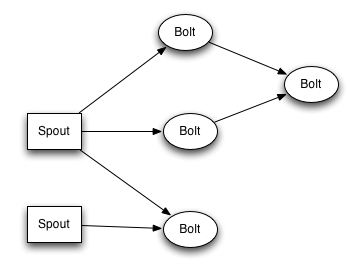
\includegraphics[scale=0.7]{images/topology.png}
\end{center}
\caption{Simple example topology}
\end{figure}
Note that every node can potentially be connected to a multitude of Bolts, both through incoming and outgoing streams (Spouts are the exception here. This is due to the different role which the Spouts play in a Topology and will be explained in the following paragraphs)

\subsection{Of Spouts, Bolts and everything in between}

Of course, the Cluster and the Topology aren't just two separate concepts working independently from each other. There is actually a connection between them, and it relies on a type of process mentioned earlier: The \textit{Supervisor}. Although the deeper functionality is much more complex and will be explained later, for now it is important to know that a Supervisor runs a multitude of threads which in turn execute the calculations for the \textit{Components}, which are, dependent on their role, called \textit{Spouts} and \textit{Bolts}.\\

As mentioned earlier, Storm was created to process streams of incoming data, and it is therefore reasonable to continue our exploration of the Cluster at the very point where the data enters it as well.

\subsubsection{Spouts}

In Storm, a Spout is the type of node in a Topology which emits one or more streams of data to every node connected to it. This data is usually provided to the Spout by an external service - a good example would be an API from any website which provides data in the form of streams. \\

It is important that every (physical) device on which a \textit{Supervisor} is run actually has access to the original source of data. This is due to the fact that the developer working with Storm has no control over the location where the Spouts and Bolts are actually run; This assignment is done by the Nimbus. It should therefore be assumed that \textit{every} physical device in the Cluster could potentially be selected to have one or more Spouts running on it. In the case of the original data source being a website, this is of course an almost negligible limitation. But if the data originates from a certain process running on a separate machine, the developer has to make the data available to the Spouts by implementing a server.\\

When talking about Spouts, there is an important distinction to make between \textit{reliable} and \textit{unreliable} Spouts. Imagine this like the difference between TCP and UDP: An unreliable Spout simply outputs data without requiring confirmation of any sort; a simple fire-and-forget implementation. A reliable Spout on the other hand provides the tools to check not only if the sent data tuple makes it to its recipient, but if the data tuple has actually completed its entire journey through the Topology. The two methods which a reliable Spout provides to that end are called \textit{ack} and \textit{fail}, which are called whenever a tuple emitted from the Spout successfully completes its journey or fails along the road.\\

Probably the most important Method of Spouts independent of their reliability is called \textit{nextTuple}. Whenever nextTuple is called on a Spout, it emits the next data tuple from its internal buffer onto every stream it is connected to.

\subsubsection{Bolts}

Unlike the Spouts, whose most difficult computational task is the acquisition of data, the Bolts are the actual workhorse of the Topology. Every Bolt needs at least some kind of data input, and this is done by \textit{subscribing} to a data stream, which may originate from either a Spout or a Bolt.\\

While the most central method of the Spout is nextTuple, the method which is most often called in Bolts is the \textit{execute} method. The execute method takes a tuple of incoming data and applies the appropriate processing step to it. It is important to note that while a Bolt's execute Method could technically be extremely powerful (the execute method is of course implemented by the developer in his/her language of choice), it is a common practice to split all aspects of the computational task which the Topology shall accomplish into adequately small steps, each of which has an own class of Bolts executing it. This is mainly due to the strong limitation that execute is called for every single data tuple separately, thereby requiring the user to limit the functionality of each Bolt in such a way that it can treat every tuple independently.\\

As mentioned before, Bolts too can emit streams of data. In order to do so, each processed data tuple is handed to an instance of the OutputCollector class which not only provides methods to emit tuples to streams but also an \textit{ack} and \textit{fail} method to indicate if said tuple has been successfully processed.

\subsubsection{Streams and Grouping}

In Storm, the streams are used to transfer data between nodes, and are defined as unboundes sequences of data tuples. By default, these data tuples can of course contain the primitive data types as well as Strings and byte arrays. Furthermore, the developer can specify a scheme that declares certain segments of each tuple as fields (Just like for example in a TCP packet, there are fields for ports, sequence number etc). It is also possible for the user to create their own serializable data type so that they can be used within Storm tuples. Each stream is identified by an id given to it upon declaration.\\

In order to understand stream grouping, one first needs to get a graps on another concept called a \textit{task}. In Storm, a task performs the actual processing of data. While all of the aforementioned information about Spouts and Bolts holds true, it is now necessary to realize that a \textit{Component} itself is not directly executed by a Supervisor: It is rather the \textit{task} which makes up the Component that is run inside a thread on the Supervisor, and the developer is able to specify the number of tasks of each Component. There is still more to say about this topic, but for now, just keep in mind that when the developer programs their Spouts and Bolts, they actually define a task for each Component which emit tuples (for Spouts) or process incoming tuples (for Bolts).\\
\indent Basically, stream grouping defines how data tuples reaching a Bolt are distributed across the tasks which make up said Bolt. There is a multitude of groupings already implemented in Storm: There is the straight-forward shuffle grouping, which sends each incoming tuple to a random task of the receiving bolt. Another important one is Fields grouping, which routes the tuples to the tasks based on the tuple's content. It is even possible for the producer of the data tuples on a stream to specify to which task of the recipient each tuple is sent.

\subsection{Arranging Tasks}

The last few paragraphs introduced a lot of terminology and concepts which may be quite confusing at a first glance. The differences between them however, while sometimes not very obvious, are important enough to be looked at in more detail, and some concept are also worth reiterating at this point.\\

First of all, it should be clarified how exactly the tasks fit into the whole picture using the following figure:\\
\begin{figure}[H]
\begin{center}
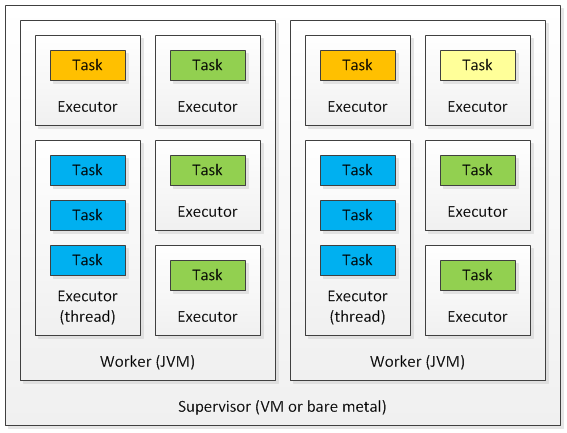
\includegraphics[scale=0.7]{images/Storm-Supervisors-Workers-Executors-Tasks.png}
\end{center}
\caption{Grouping of Supervisor subunits}
\end{figure}
We can see that the whole thing depicts a Supervisor daemon which is run on a node in the Cluster, thereby identifying that node as a worker node. The Supervisor then can run one or more Worker processes, each of which is running in its own JVM.\\
\indent Now comes the interesting part: As mentioned in the last chapter, each Component (Spout or Bolt) has a certain amount of Tasks specified (by the developer) which execute said Component's computations. It is worth noting now, however, that a Task itself is not a thread, but instead is run inside an \textit{Executor} thread. While an Executor can run an arbitrary number of tasks, it is generally recommended to have each task running on its own Executor.\\
\indent In this illustration, the colour of each Task specifies to which Component it belongs; In this case, the blue Tasks might belong to the Spout called BlueSpout, the green Tasks to the Bolt GreenBolt etc. As a clarification: Every Task of a certain Component runs the exact same code. This is the code specified by the developer, for example in the \textit{execute}-Method of a Bolt.\\
\indent Another important thing to note is that no Executor runs Tasks from more than one Component.

\subsubsection{Parallelism and grouping Tasks into Executors}

So far, we have mainly covered the main aspects of the Supervisors - running a certain number of workers, specifying Components and on how many Tasks they run their computations - but the actual functionality of the Nimbus pretty much remained a mystery. The observant reader however might have noticed that especially in the topics covered in these last few paragraphs, the Nimbus has been very active behind the scenes: All kinds of administrative work like assigning Workers to Supervisors, grouping Tasks into Executors and Executors into Workers is actually done by the Nimbus.\\
\indent Assignment of the Workers is rather straight forward; the Nimbus tends to distribute these evenly across its Supervisors and make changes if necessary. For the rest, there is one last important concept called \textit{Parallelism hint}, which is best explained using another illustration from Storm's website:\\
\begin{figure}[H]
\begin{center}
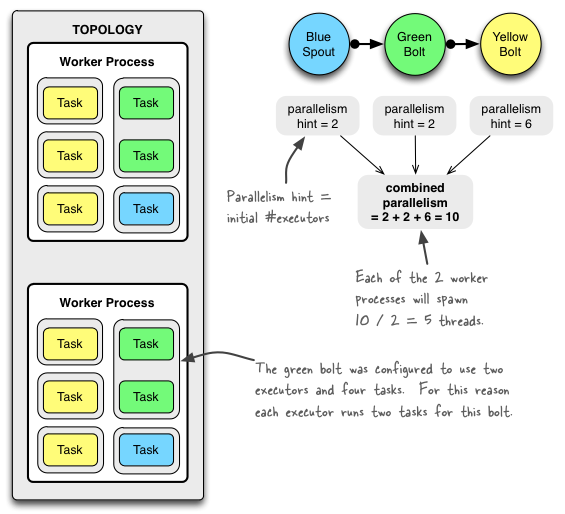
\includegraphics[scale=1]{images/example-of-a-running-topology.png}
\end{center}
\caption{The concept of parallelism}
\end{figure}
Not explicitly stated is the fact that the blue Spout has been specified to be run on two Tasks, the green Bolt on four and the yellow Bolt on six. By also defining a parallelism hint, the Nimbus now has all the information it needs to evenly distribute the tasks among their respective Executors, and assign these Executors to the Worker processes.
%                Simon's Part
%-------------------------------------------------------------------------------------------------------------
%-------------------------------------------------------------------------------------------------------------
%-------------------------------------------------------------------------------------------------------------
%-------------------------------------------------------------------------------------------------------------
%-------------------------------------------------------------------------------------------------------------
\section{Implementation}
\subsection{Programming Languages}
Storm, having it's Workers running on a Java Virtual Machine, offers extensive support for Java is best used in an application written in Java. If the developer is, however, hard-pressed on using a different language, Storm by default supports integration of the programming languages \textit{Python}, \textit{Fancy} and \textit{Ruby} into Java code via ShellBolts and -Spouts. So the usage of a Bolt written in Python might look like this:\\
\begin{lstlisting}
public static void SplitSentence extends ShellBolt
                                 implements IRichBolt {
                                 
    public SplitSentence() {
        super("python", "splitsentence.py");
    }
    
    public void declareOutputFields(
            OutputFiledDeclarer declarer) {
        declarer.declare(new Fields("word"));
    }
    
}
\end{lstlisting}
\subsection{Spouts and Bolts in Java}
\label{sec:ImplementComponents}
Java is an object oriented language, and as such the components of a topology are objects. In order to define a Spout or Bolt, the developer can either extend a pre-existing Bolt or Spout class or directly implement an interface. Storm provides the classes \textit{BaseRichBolt} and \textit{BaseRichSpout} as well as the interfaces \textit{IRichBolt} and \textit{IRichSpout} for the user to build off of.\\

The processing logic of the component is then defined in a function \lstinline$public void nextTuple()$ for Spouts and \lstinline$public void execute(Tuple tuple)$ for Bolts. The function \textit{execute} will be called whenever the Bolt receives a tuple and be given that tuple as a parameter, while the \textit{nextTuple} function will be called as often as the hardware allows. Should this not be desired, it is advised that the developer lets the function terminate without taking action until an action is to be taken rather than letting it sleep, as Storm calls all the Spout methods on the same thread.

A simple implementation of a Spout and Bolt may look like this:
\begin{lstlisting}
public class MySpout extends BaseRichSpout {
    @Override
    public void nextTuple() {
        String output = "some data";
        _collector.emit(new Values(output));
    }
}

public class MyBolt extends BaseRichBolt {
    @Override
    public void execute(Tuple tuple)
        int output = someFunction(tuple.getInteger(0));
        _collector.emit(tuple, new Values(output));
        _collector.ack(tuple);
    }
}
\end{lstlisting}
\subsection{Topologies in Java}
\label{sec:ImplementTopology}
In order to combine the Bolts and Spouts created in \ref{sec:ImplementComponents} into a functioning topology, one needs to start with a TopologyBuilder object provided by Storm. This object can add components to the topology by calling the function \textit{setSpout} and \textit{setBolt}, which take a component object as well as a number describing how many instances of these components are to be running in parallel in the network. These components can then be linked via a set of grouping functions that define which components will receive which component's emitted tuples as an input stream.\\

A simple topology might look like this:
\begin{lstlisting}
TopologyBuilder builder = new TopologyBuilder();
builder.setSpout("sentences", new RandomSentenceSpout(), 5);
builder.setBolt("split", new SplitSentence(), 8)
    .shuffleGrouping("sentences");
builder.setBolt("count", new WordCount(), 12)
    .fieldsGrouping("split", new Fields("word"));
\end{lstlisting}
Which will generate a topology such as this:\\

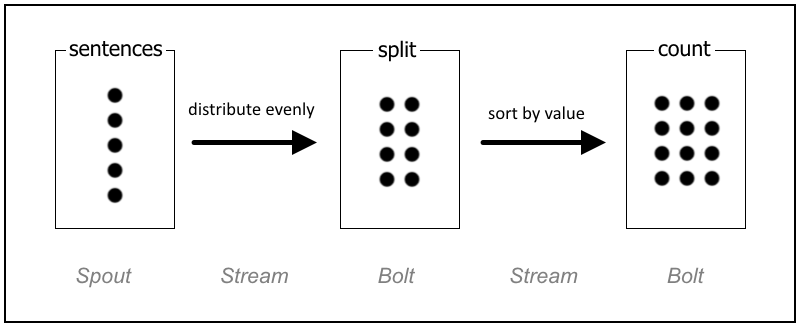
\includegraphics[width=\textwidth]{images/WordCountGraph.png} 

\subsection{Clusters in Java}
\label{sec:ImplementCluster}
As with everything else, Storm clusters in Java are represented as objects. Once the topology is defined as specified in \ref{sec:ImplementTopology}, it can be submitted to a cluster along with a configuration object that defines certain things like the number of workers to be distributed throughout the network.\\

A simple cluster might look like this:
\begin{lstlisting}
Config conf = new Config();
conf.setNumWorkers(2);
DistributedCluster cluster = new DistributedCluster();
cluster.submitTopology("someID", conf,
    builder.createTopology());
\end{lstlisting}
%                Phillip's Part
%-------------------------------------------------------------------------------------------------------------
%-------------------------------------------------------------------------------------------------------------
%-------------------------------------------------------------------------------------------------------------
%-------------------------------------------------------------------------------------------------------------
%-------------------------------------------------------------------------------------------------------------
\section{Apache Storm Setup}
The following 4 steps demonstrate how to setup an Apache Storm Cluster
\subsection{Setup a Zookeeper Cluster}
Depending on how big the Storm Cluster will be the number of Supervisor nodes has to be determined. In cases of small clusters it is sufficient to have a Zookeeper cluster with one Zookeeper server only.
The Apache Zookeeper server can be found under the following \href{http://www.eu.apache.org/dist/zookeeper/stable/}{link}. The config file in \path{zookeper/conf/zoo_sample.cfg} should be checked and the following two lines appended, to prevent running out of disk space.
\begin{verbatim}
autopurge.purgeInterval=24
autopurge.snapRetainCount=5  
\end{verbatim}
The server can be started afterwards by running the following script: \path{zookeper/bin/zkServer[.cmd|.sh]}
\subsection{Install dependencies}
Apache Storm has some dependencies for software versions of the Supervisor nodes:
\begin{verbatim}
Java 6
Python 2.6.6
\end{verbatim}
Although some testing has shown that it is also running with newer versions of Java.
\subsection{Nimbus and Supervisor nodes}
The next step includes downloading a distribution of Apache Storm (\href{http://storm.apache.org/downloads.html}{link}) onto the devices which will run the Nimbus server and the Supervisor clients.
In order to establish a connection between them and the Zookeeper, the config file in \path{apache-storm/conf/storm.yaml} has to be changed accordingly. The two attributes \verb!storm.zookeeper.servers! and \verb!nimbus.host! have to be set to the IP addresses of the corresponding devices. In case of the Nimbus device they have to be set to "localhost". The attribute storm.local.dir has to be set to some path indicating a directory where Storm can store data locally.
\subsection{Setting up Supervisor}
Apache Storm is a fail fast system, which means that it exits if there are any exceptions thrown. To make it run more stable a supervisory program can be used. It basically observes the Nimbus and Supervisor process and restarts them if they break down. A possible software solution would be Supervisor, a process control system, which runs only on UNIX-like operating systems. Download: \href{http://supervisord.org/#}{link}.
To set it up after installation the following lines have to be appended to \path{/etc/supervisord.conf}
\begin{verbatim}
[program:storm-nimbus]
command=/usr/local/storm/bin/storm nimbus
user=storm
autostart=true
autorestart=true
startsecs=10
startretries=999
log_stdout=true
log_stderr=true
logfile=/var/log/storm/nimbus.out
logfile_maxbytes=20MB
logfile_backups=10
\end{verbatim}
The command and logfile path as well as the program name have to be changed accordingly. After setting up the configuration file the supervisor daemon (which is a component of the supervisory program not to be confused with the Supervisor process running on the node) has to be started with: 
\begin{verbatim}
sudo service supervisord start
\end{verbatim}
For troubleshooting:
\begin{verbatim}
sudo supervisorctl status
\end{verbatim}
The sample configuration is from this \href{http://www.michael-noll.com/tutorials/running-multi-node-storm-cluster/#install-supervisord}{site}. The page also holds lots of useful information on setting up Apache Storm clusters.
\subsection{Deploying topologies}
After the explanation on how to create a cluster in \ref{sec:ImplementCluster}, the following part describes how to get said cluster deployed and running.\\
First the coded cluster has to packed with all its packages into a jar file. It is rather important to include only libraries into the jar which are not from Apache Storm, since including these libraries will end up in a topology which is not deployable. After successfully packing the topology jar, it can be submitted to the running Storm Cluster via the storm client:
\begin{verbatim}
storm jar path/to/allmycode.jar org.me.MyTopology arg1 arg2 arg3
\end{verbatim}
More information on how to deploy a topology and troubleshooting can be found  \href{http://storm.apache.org/documentation/Running-topologies-on-a-production-cluster.html}{here}:
\section{Sources}
\begin{itemize}
\item \url{http://storm.apache.org/documentation.html}
\item \url{http://www.michael-noll.com/tutorials/running-multi-node-storm-cluster/}
\end{itemize}
\begin{description}
\item[Figure 1] \url{http://storm.apache.org/tutorial.html}
\item[Figure 3] \url{http://storm.apache.org/documentation/Understanding-the-parallelism-of-a-Storm-topology.html}
\end{description}
\end{document}